\chapter{Stand der Wissenschaft}
Diese Kapitel soll dem Leser eine Übersicht über den aktuellen Stand der Wissenschaft geben. Zu diesem Zweck hat dieses Kapitel zwei Teile. Im ersten Teil wird zunächst grundlegend die Funktionsweise von CNNs erläutert. Im zweiten Teil des Kapitels wird ein Überblick über die bisherigen wissenschaftlichen Erkenntnisse im Themenbereich dieser Arbeit vorgetellt.
\section{Funktionsweise eines CNNs}\label{sec:conv}
Die Quelle für dieses Unterkapitel ist soweit nicht anders vermerkt ein Buch über \enquote{Deep Learning} \cite{CNNBook}.

CNNs sind spezielle neuronale Netze. Der Unterschied zu einem \enquote{Multilayer-Perzeptron (MLP)\footnote{Die Hintergründe des MLPs und allgemein neuronaler Netzwerke werden hier nicht behandelt. Für eine Einführung in neuronale Netzwerke kann aber \cite{neural} herangezogen werden}} ist, dass bei einem MLP jede Verbindung zwischen Neuronen und die Neuronen selber ein eigenes trainierbares Gewicht haben. Aus diesen trainierbaren Werten wird mittels einer Matrixmultiplikation mit den Eingabedaten bzw. den Daten der vorherigen Schicht die Ausgabe jedes Neurons berechnet.
Im Gegensatz dazu sind CNNs neuronale Netze, die in mindestens einer ihrer Schichten die Faltung anstelle der allgemeinen Matrixmultiplikation verwenden.


Dies bedeutet, dass die Eingabedaten für ein CNN für diese Faltung geeignet sein müssen. Geeignet für die Faltung sind Eingabedaten, die gridförmig angeordnet sind. Bilddaten sind ein grosser Anwendungsbereich für CNNs.

Bei der Faltung wird auf die Eingabedaten bzw- die Daten dr vorherigen Schicht ein Kernel angewendet.

In Abbildung \ref{fig:faltung} ist zu sehen wie die Faltung auf einem Bild durchgeführt wird. Der Kernel wird auf jedes Teilbild mit der Grösse des Kernels angewendet. Die korrespondierenden Felder werden multipliziert und alle entstehenden Produkte werden addiert. So entsteht aus der Faltung des Kernels mit der Eingabe in die entsprechende Schicht eine Featuremap.
Mehrere dieser Kernel bilden zusammen ein Convolutional Layer. \todo[inline]{bis hier}

\begin{figure}[h]
 \centering
 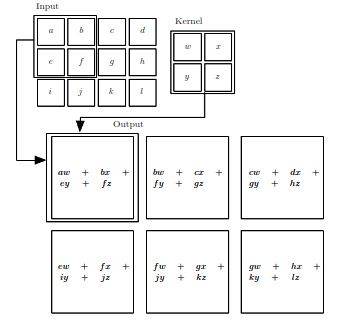
\includegraphics[width=0.45 \textwidth,keepaspectratio=true]{images/convolution.png}
 % convolution.png: 342x321 px, 72dpi, 12.06x11.32 cm, bb=0 0 342 321
 \label{fig:faltung}
 \caption{Definition der Faltung \cite{CNNBook}}
\end{figure}

In einem CNN werden mehrere dieser Convolutional Layer hintereinander geschaltet, um komplexe Features erkennen zu können. 



Eine beispielhafte Übersicht über die CNN-Architektur ist in Abbildung \ref{fig:cnn} zu sehen.


\begin{figure}[h]
  \centering
  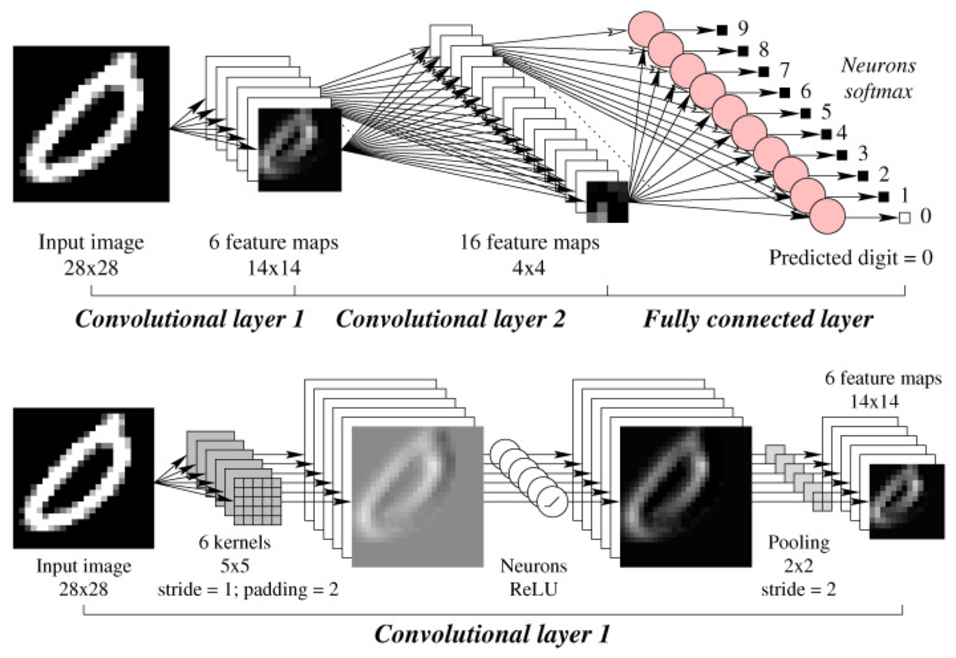
\includegraphics[width=0.75\textwidth]{images/cnn.pdf}
  \caption{Convolutional Neural Net \cite{CNNImg}}
  \label{fig:cnn}
\end{figure}

In Abbildung \ref{fig:cnn} ist zu sehen, dass ein CNN aus hintereinander geschalteten Conv-Layer besteht. Die Funktion der Conv-Layer wird nun näher betrachtet.

Wie in Abbildung \ref{fig:cnn} zu sehen ist, ist ein Conv-Layer die hintereinander Schaltung verschiedener Operationen:
\begin{itemize}
 \item Faltung des Eingabebildes mit dem Kernel
 \item Anwendung der Aktivierungsfunktion ReLU
 \item Pooling
\end{itemize}

Abbildung \ref{fig:cnn} beinhaltet auch noch die Begriffe Stride und Padding, welche für das Verstehen dieser Arbeit zwar nicht notwendig sind, hier der Vollständigkeit halber trotzdem erklärt werden. 

Padding löst das Problem, das entsteht, wenn der Mittelpunkt des Filters auf ein Pixel im Randbereich gelegt wird. Hier taucht das Problem auf, dass der Filter auch auf nicht vorhandenen Pixeln aufliegt und die Filteroperation hier somit nicht definiert ist. Padding setzt nun den Rand fort oder belegt diesen Rand mit einem festgelegten Wert, um dort eine gültige Filteroperation zu erzeugen. 

Stride ist der Parameter, der bestimmt um wie viele Felder der Filter nach der Anwendung verschoben werden soll. Bei größerem Stride kann die entstehende Feature-Map verkleinert werden.

Pooling ist eine Operation, die die Größe der Feature-Map verkleinert und somit Overfitting vermeidet.

Die Fully-Connected-Layer errechnen aus den Ausgängen der Convolutional-Layer, in welche Klasse ein Objekt klassifiziert werden soll.  

Die Filter, die auf die Feature Maps bzw. die Eingabebilder angewendet werden, sind trainierbar. Zusätzlich sind auch die Gewichtungen des Fully-Connected Layers trainierbar. Das heißt durch den Trainingsprozess wird versucht die Werte in der Filtermatrix und des Fully-Connected Layer so zu verändern, dass das gesamte CNN besser klassifizieren kann. Für diese Veränderung wird ein Gradientenabstiegsverfahren, welches rückwärts durch die Schichten propagiert wird, benutzt.



\section{Überblick über die gängigen Methoden}
\todo[inline]{kurzer Sectioneinleitungstext über die gängigen Methoden}
